\documentclass{beamer}
\usetheme{Hannover}
\usepackage{fontspec, xunicode, xltxtra}
\XeTeXlinebreaklocale "zh"
\XeTeXlinebreakskip = 0.1pt plus 1pt minus 0.1pt
\usepackage{xeCJK} 
\usepackage{fontspec}  
\setCJKmainfont{SimSun} 
\setCJKmonofont{SimSun} 
\setmainfont{Courier}%{Times New Roman} {SourceCodePro-Regular}{Consolas}{Courier}
\usepackage{hyperref}
\usepackage[utf8]{inputenc} % this is needed for german umlauts
\usepackage[english]{babel} % this is needed for german umlauts
\usepackage[T1]{fontenc}    % this is needed for correct output 
                            % of umlauts in pdf
\usepackage{pgf,pgfarrows,pgfnodes,pgfautomata,pgfheaps}
\usepackage{amsmath,amssymb}
\usepackage{graphicx}
\usepackage{multimedia}
\usepackage{listings}
\lstset{language=C++}
\lstset{breaklines}
\lstset{extendedchars=false}

\begin{document}
\title{数据结构大作业报告}
\subtitle{八数码}
\author{姚皓天}
\date{2014年11月}
\subject{数据结构}

\frame{\titlepage}
\begin{frame}
\section{基本原理}
\subsection{概述}
\begin{block}{概述}
本程序采用Microsoft Visual Studio 2012 的“MFC应用程序”开发,实现了简单地八数码的搜索算法和演示功能。实现了三种算法,深搜、广搜、和A*算法。因为程序功能有限,使用了基本的单对话框模板实现程序功能。\par
在MFC的基本框架之上,首先编写了EightFigureState类,用于统一使用一个int变量来描述八数码的的状态,同时还保存搜索中产生的相关信息。SearchCore类作为作为基类派生所有的搜索方法。CEightFigureDlg类用于控制图形界面。
\end{block}
\end{frame}

\begin{frame}
\subsection{特色}
\begin{block}{特色}
\begin{itemize}
\item 使用SearchCore类作为作为基类,派生出所有的搜索方法,每个方法复写虚函数Search,使用统一的接口,方便编程与扩展。
\item 开发过程中使用了VS的单元测试框架对几个重要类的方法进行了测试,大大提高了开发成功率,缩短了开发时间。
\item 搜索中访问过的状态使用Hash Set保存,可以取得很快的速度。
\end{itemize}
\end{block}
\end{frame}

\begin{frame}
\subsection{界面}
\begin{figure}[H]
\centering
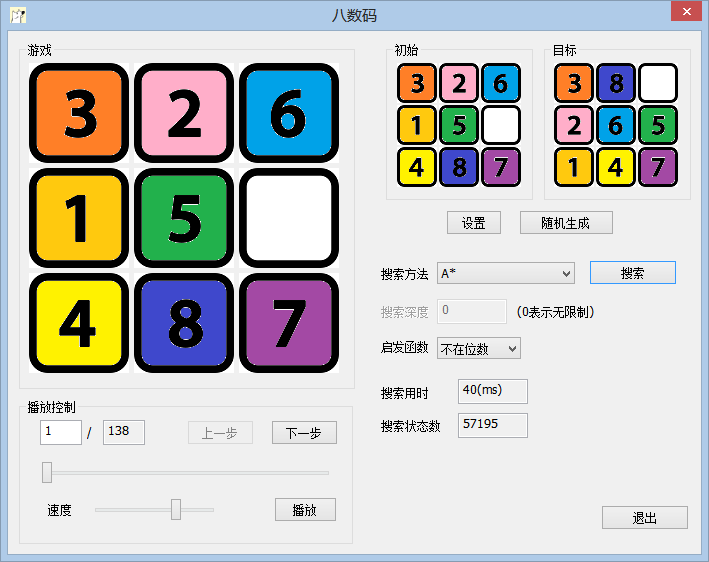
\includegraphics[width=0.6\textwidth]{1.png}
\caption{界面} 
\end{figure}
\end{frame}

\begin{frame}
\section{程序设计}
\subsection{概要设计}
\begin{block}{概要设计}
在MFC的基本框架之上,首先编写了EightFigureState类,用于统一使用一个int变量来描述八数码的的状态,同时还保存搜索中产生的相关信息。SearchCore类作为作为基类派生所有的搜索方法。CEightFigureDlg类用于控制图形界面。
\begin{figure}[H]
\centering
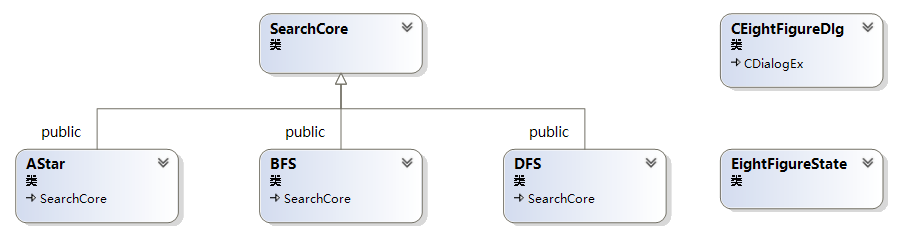
\includegraphics[width=0.8\textwidth]{3.png}
\caption{类图} 
\end{figure}
\end{block}
\end{frame}

\begin{frame}
\section{设计心得}
\begin{block}{单元测试}
\begin{figure}[H]
\centering
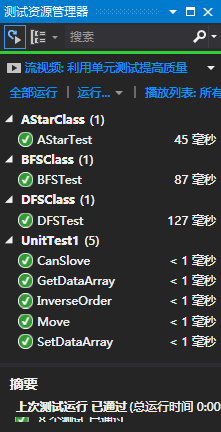
\includegraphics[scale = 0.5]{2.png}
\caption{单元测试} 
\end{figure}
\end{block}
\end{frame}

\end{document}